\documentclass[12pt,a4paper]{article}
\usepackage[utf8]{inputenc}
\usepackage[T1]{fontenc}
\usepackage{times}
\usepackage[margin=2.5cm]{geometry}
\usepackage{setspace}
\doublespacing
\usepackage{graphicx}
\usepackage{booktabs}
\usepackage{natbib}
\usepackage{hyperref}
\usepackage{amsmath}

\title{Volcanic Informedness: Evidence for Volcanically-Aware Cultural Practices in Java and Bali}

\author{Mukhlis Amien\textsuperscript{1} \and Go Frendi Gunawan\textsuperscript{1}}

\date{}

\begin{document}

\maketitle

\noindent\textsuperscript{1}Lab Data Sains, Universitas Bhinneka Nusantara, Malang, Indonesia

\vspace{1em}
\noindent\textbf{Corresponding author:} Mukhlis Amien (\texttt{mukhlis.amien@ubhara.ac.id})

\begin{abstract}
Java and Bali host 45 active volcanoes and over 74,000 years of continuous human habitation. We investigate whether this sustained volcanic exposure left detectable traces in local cultural practices---a phenomenon we term \emph{volcanic informedness}. Using five independent computational tests, we find that (1) Hindu-Buddhist temples (\emph{candi}) cluster preferentially on western flanks of volcanoes (Rayleigh $p=3.4\times10^{-8}$, $n=142$), consistent with tephra-sheltered positioning during southeast monsoon eruptions; (2) Zone A ($<$10~km from volcanic peaks) is overrepresented by 17.9$\times$ compared to random placement; (3) the traditional Javanese agricultural calendar Pranata Mangsa inadvertently encodes volcanic hazard seasonality, with peak eruption density during its wet-season month Kapitu (3.8$\times$ the lowest month; chi-squared $p=0.042$); (4) these patterns are local rather than universal---a cross-cultural test across 116 Austronesian societies finds no global correlation between volcanic proximity and ritual complexity ($p=0.973$); and (5) toponymic analysis of 25,244 Javanese villages reveals that court-center Indianization, not volcanic proximity, drives cultural overwriting (Spearman $\rho=0.387$, $p<0.0001$). We argue that volcanic informedness represents practical environmental knowledge encoded in architecture and calendar rather than population-level cultural selection. This local phenomenon has been overlooked because archaeological models emphasize external cultural inputs over endogenous landscape adaptation.

\vspace{0.5em}
\noindent\textbf{Keywords:} volcanic informedness, Java, Bali, candi, Pranata Mangsa, cultural ecology, traditional ecological knowledge, taphonomic bias
\end{abstract}

\newpage

% ============================================================
\section{Introduction}
% ============================================================

\subsection{Volcanic Landscapes and Cultural Adaptation}

Java is the world's most densely populated volcanic island, home to 34 of Indonesia's 127 active volcanoes \citep{gvp2023}. Together with Bali's Agung and Batur, these 45 volcanic systems have erupted on average once every 1--2 years over the historical record, making the Java--Bali arc arguably the most volcanically active continuously inhabited region on Earth.

The dominant narrative of Javanese cultural history, however, has been shaped almost entirely by external influences: Indianization (1st--15th centuries CE), Islamization (15th--17th centuries), and European colonization (17th--20th centuries). The role of the volcanic landscape itself---not merely as a backdrop, but as an active shaping force on cultural practices---has received remarkably little systematic attention. Individual studies have noted volcanic imagery in Javanese cosmology \citep{headley2004}, the agricultural significance of volcanic soils \citep{mohr1938}, and the disaster-response patterns of volcanic communities \citep{schlehe1996}, but no study has tested whether the cumulative effect of living near active volcanoes left statistically detectable signatures in architecture, calendrical systems, or land-use decisions.

We address this gap through what we term \emph{volcanic informedness}: the encoding of practical volcanic knowledge in cultural practices by communities living near active volcanoes. Unlike the stronger claim of Volcanic Cultural Selection (VCS)---which would require differential survival of volcanic vs.\ non-volcanic communities---volcanic informedness requires only that communities \emph{observe} and \emph{encode} volcanic patterns, whether intentionally or as a structural byproduct of environmental adaptation.

\subsection{Defining Volcanic Informedness}

Volcanic informedness sits within the broader framework of Traditional Ecological Knowledge (TEK), defined as ``a cumulative body of knowledge, practice, and belief, evolving by adaptive processes and handed down through generations by cultural transmission, about the relationship of living beings with one another and with their environment'' \citep{berkes2018}. What distinguishes volcanic informedness from general TEK is the specific volcanic hazard dimension: communities encode knowledge not only about soil fertility, rainfall, and growing seasons, but also---perhaps inadvertently---about eruption timing, tephra dispersal patterns, and lahar pathways.

We propose three criteria for detecting volcanic informedness computationally:
\begin{enumerate}
    \item \textbf{Spatial criterion:} Cultural features (architecture, land use) show non-random distributions relative to volcanic peaks, in directions predicted by known eruption dynamics.
    \item \textbf{Temporal criterion:} Calendrical or seasonal practices correlate with volcanic hazard seasonality beyond what agricultural adaptation alone would predict.
    \item \textbf{Locality criterion:} The patterns are local to volcanically active regions, not a universal correlate of volcanic proximity across diverse cultures.
\end{enumerate}

\subsection{Scope and Limitations}

This paper makes a deliberately \emph{local} claim about Java and Bali. A cross-cultural test (Section~\ref{sec:crosscultural}) demonstrates that volcanic informedness does not generalize to a pan-Austronesian phenomenon. We present only computational evidence; ethnographic validation through fieldwork interviews with volcanic communities (Tengger, Bali Aga) remains a priority for future work. This study complements the VOLCARCH project's demonstration that volcanic sedimentation creates systematic biases in the archaeological record \citep{amien2026p1}, and that pre-Indic cultural elements survive differentially in peripheral regions \citep{amien2026p9}: the same volcanoes that \emph{bury} evidence of past civilizations also \emph{shaped} the cultural practices of those civilizations.

% ============================================================
\section{Study Area and Data}
% ============================================================

\subsection{Volcanic Landscape of Java and Bali}

The Java--Bali volcanic arc contains 45 Holocene-active volcanoes spanning the island's 1,000~km length \citep{whitten1996, thouret1999}. Major systems include Merapi (central Java, pyroclastic-dominated), Kelud (east Java, lahar-dominated), Semeru (persistent Strombolian activity), the Tengger caldera complex (including Bromo), and Agung--Batur in Bali. Eruption frequency across the arc averages 10--15 events per decade \citep{gvp2023}.

A critical meteorological factor is the dominance of the southeast monsoon during eruption season: prevailing winds carry volcanic tephra predominantly westward and northwestward during the wet season (November--March), when eruption frequency peaks (Section~\ref{sec:calendar}). This asymmetric dispersal creates a natural ``sheltered'' zone on western volcanic flanks.

\subsection{Candi Dataset}

We compiled coordinates for 142 Hindu-Buddhist temples (\emph{candi}) across Java from published archaeological surveys and the regional heritage authority (BPCB Jawa Timur), building on the architectural catalogues of \citet{dumarcay1993} and \citet{soekmono1995}. For each candi, we identified the nearest active volcano and computed the haversine distance and bearing. Additionally, 20 candi have documented entrance orientations from published architectural studies, enabling a separate test of facing direction.

The dataset is dominated by Penanggungan (73 candi, 51\% of total), a sacred mountain in East Java that has hosted religious activity since at least the 10th century CE. We analyze Penanggungan both as part of the full dataset and separately to control for single-mountain effects.

\subsection{Eruption Seasonality Data}

From the Global Volcanism Program \citep{gvp2023}, we extracted 127 eruptions with known start months from four major Java volcanoes: Kelud (32 events), Merapi (47 events), Semeru (28 events), and Tengger-Bromo (20 events). Each eruption was mapped to the corresponding Pranata Mangsa month following the Gregorian--Pranata Mangsa correspondence table of \citet{daldjoeni1984}. We note that the Merapi dataset has potential reporting gaps in the GVP seasonal record.

\subsection{Cross-Cultural Comparative Data}

For the locality test, we used the Pulotu Database of Pacific Religions \citep{watts2015}, which provides standardized ethnographic variables for 116 Austronesian societies. We computed each society's haversine distance to the nearest Holocene-active volcano from the GVP database (854 volcanoes worldwide) and tested for correlations with nine ritual and cooperation variables.

\subsection{Toponymic Data}

Village names for 25,244 settlements across Java were obtained from the Indonesian Central Bureau of Statistics (BPS) via the \emph{cahyadsn/wilayah} dataset (Kepmendagri 2025, MIT license). Each village name was classified into linguistic layers (Pre-Hindu, Sanskrit, Arabic, Mixed, or Unknown) using morpheme-based dictionaries, following the methodology described in the supplementary materials.

% ============================================================
\section{Methods}
% ============================================================

\subsection{Test 1: Candi Spatial Analysis}
\label{sec:spatial}

For each of the 142 candi, we computed the azimuth from the candi to its nearest volcanic peak and the azimuth from the peak to the candi. We tested for directional clustering using:
\begin{itemize}
    \item \textbf{Rayleigh test} for circular non-uniformity (sensitive to unimodal clustering)
    \item \textbf{Quadrant chi-squared test} comparing observed N/E/S/W distribution to expected 25\% per quadrant
    \item \textbf{Zone classification}: Zone A ($<$10~km), Zone B (10--30~km), Zone C ($>$30~km), compared to expected counts under random 2D placement (area-proportional: expected $\propto r^2$)
\end{itemize}

For the 20 candi with known entrance orientation, we tested whether entrance direction faces the nearest volcano (angular difference $<$45\textdegree) vs.\ random expectation (25\%).

\subsection{Test 2: Calendar--Eruption Seasonality}
\label{sec:calendar}

We mapped each of 127 eruptions to the Pranata Mangsa calendar month in which it began. To account for the unequal length of Pranata Mangsa months (23--43 days), we computed eruption density per 30-day equivalent. We tested for non-uniform distribution using chi-squared and Rayleigh tests.

\subsection{Test 3: Cross-Cultural Falsification}
\label{sec:crosscultural}

Using Pulotu data for 116 Austronesian societies, we performed three sub-tests:
\begin{itemize}
    \item \textbf{E039a (binary):} Mann-Whitney U comparing ritual complexity on volcanic vs.\ non-volcanic islands
    \item \textbf{E039b (continuous):} Spearman correlation between distance to nearest volcano and ritual complexity
    \item \textbf{E039c (subsistence):} Test whether significant correlations reflect volcanic fertility (demographics) rather than cultural selection
\end{itemize}

\subsection{Test 4: Toponymic Overwriting Analysis}
\label{sec:toponymic}

We classified 25,244 Java village names into linguistic layers and computed the pre-Hindu ratio (Pre-Hindu names / [Pre-Hindu + Sanskrit names]) for each of 115 \emph{kabupaten} (regencies). We tested two competing hypotheses:
\begin{itemize}
    \item \textbf{H1 (volcanic):} Pre-Hindu toponyms survive more in volcanically active areas (volcanic preservation or isolation)
    \item \textbf{H2 (court-center):} Pre-Hindu toponyms survive more in areas distant from historical court centers (cultural overwriting)
\end{itemize}

\subsection{Test 5: Candi--Toponym Cross-Reference}
\label{sec:crossref}

We merged the candi dataset (Test 1) with the toponymic dataset (Test 4) by assigning each candi to its nearest \emph{kabupaten}. We tested whether \emph{kabupaten} containing candi have higher or lower pre-Hindu toponymic ratios than those without candi, using Mann-Whitney U.

% ============================================================
\section{Results}
% ============================================================

\subsection{Candi Cluster on Western Volcanic Flanks}

The 142 candi show highly non-random directional distribution relative to their nearest volcanoes. The mean azimuth from volcano to candi is 279\textdegree\ (west), with significant clustering (Rayleigh test: $\bar{R}=0.348$, $z=17.19$, $p<10^{-6}$).

The quadrant distribution is dramatically asymmetric: West 47.2\%, South 26.8\%, North 22.5\%, East 3.5\% (chi-squared $=54.68$, $p<0.0001$). The eastern quadrant is nearly empty, with only 5 candi out of 142 ($<$4\%).

\subsubsection{Zone A Overrepresentation}

When classified by distance zones, candi show extreme overrepresentation in the high-risk volcanic zone:

\begin{table}[h]
\centering
\caption{Candi distribution across volcanic proximity zones}
\begin{tabular}{lrrrr}
\toprule
Zone & Observed & Expected (random) & Ratio & Interpretation \\
\midrule
Zone A ($<$10 km) & 60 (42.3\%) & 3.4 & 17.9$\times$ & \textbf{Massive overrepresentation} \\
Zone B (10--30 km) & 65 (45.8\%) & 27.0 & 2.4$\times$ & Overrepresented \\
Zone C ($>$30 km) & 17 (12.0\%) & 111.6 & 0.15$\times$ & Underrepresented \\
\bottomrule
\end{tabular}
\label{tab:zones}
\end{table}

Chi-squared test: $\chi^2=1091.28$, $p<10^{-6}$. Under random 2D placement (area-proportional expectation), Zone A should contain only $\sim$3 candi; we observe 60.

\begin{figure}[ht]
\centering
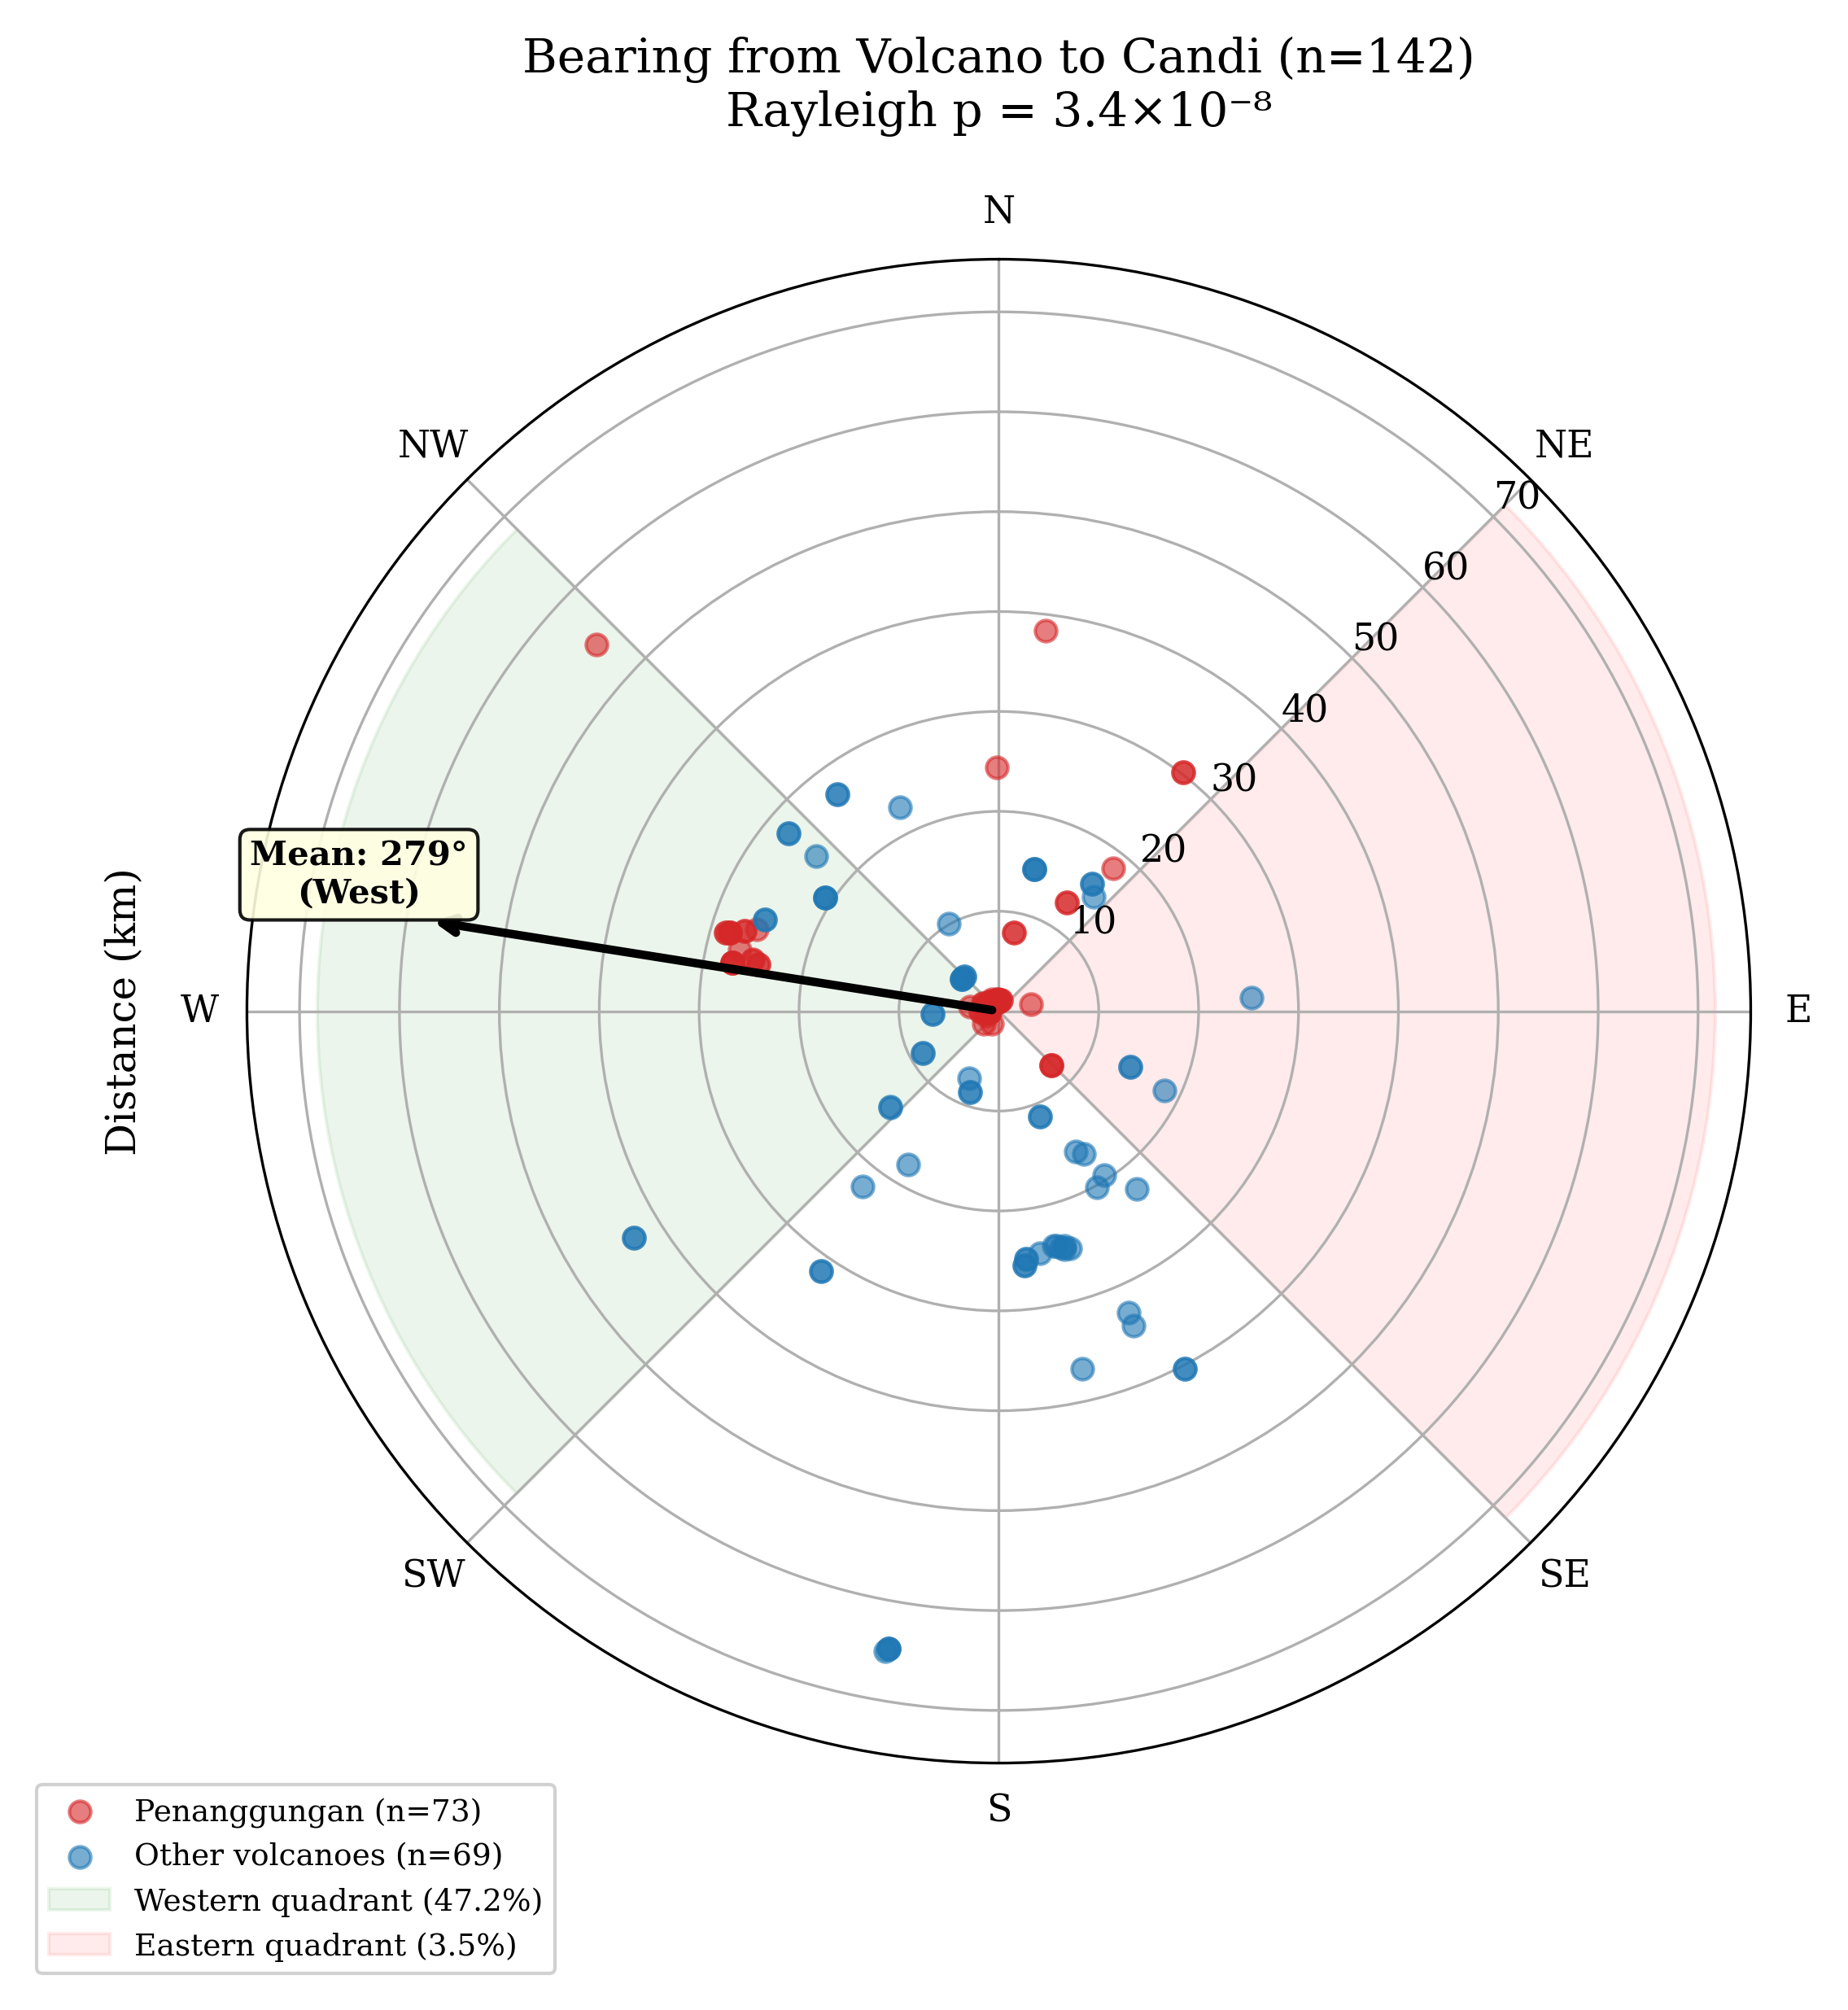
\includegraphics[width=0.7\textwidth]{figures/fig1_candi_polar_bearings.png}
\caption{Polar plot of bearings from volcanic peaks to candi ($n=142$). Distance from center represents distance in km. Green shading marks the western quadrant (47.2\% of candi); red shading marks the nearly empty eastern quadrant (3.5\%). Red dots: Penanggungan candi; blue dots: other volcanoes. Mean bearing 279\textdegree\ (west). Rayleigh $p=3.4\times10^{-8}$.}
\label{fig:polar}
\end{figure}

\subsubsection{Penanggungan Sacred Mountain}

Penanggungan alone hosts 73 candi (51\% of the dataset). Of these, 46 are on the western side (63.0\%; binomial test against $p=0.25$: $p<10^{-6}$). Even excluding Penanggungan, the remaining 69 candi still show significant directional clustering (Rayleigh $p=0.0009$), confirming that western preference is not solely a Penanggungan effect.

\begin{figure}[ht]
\centering
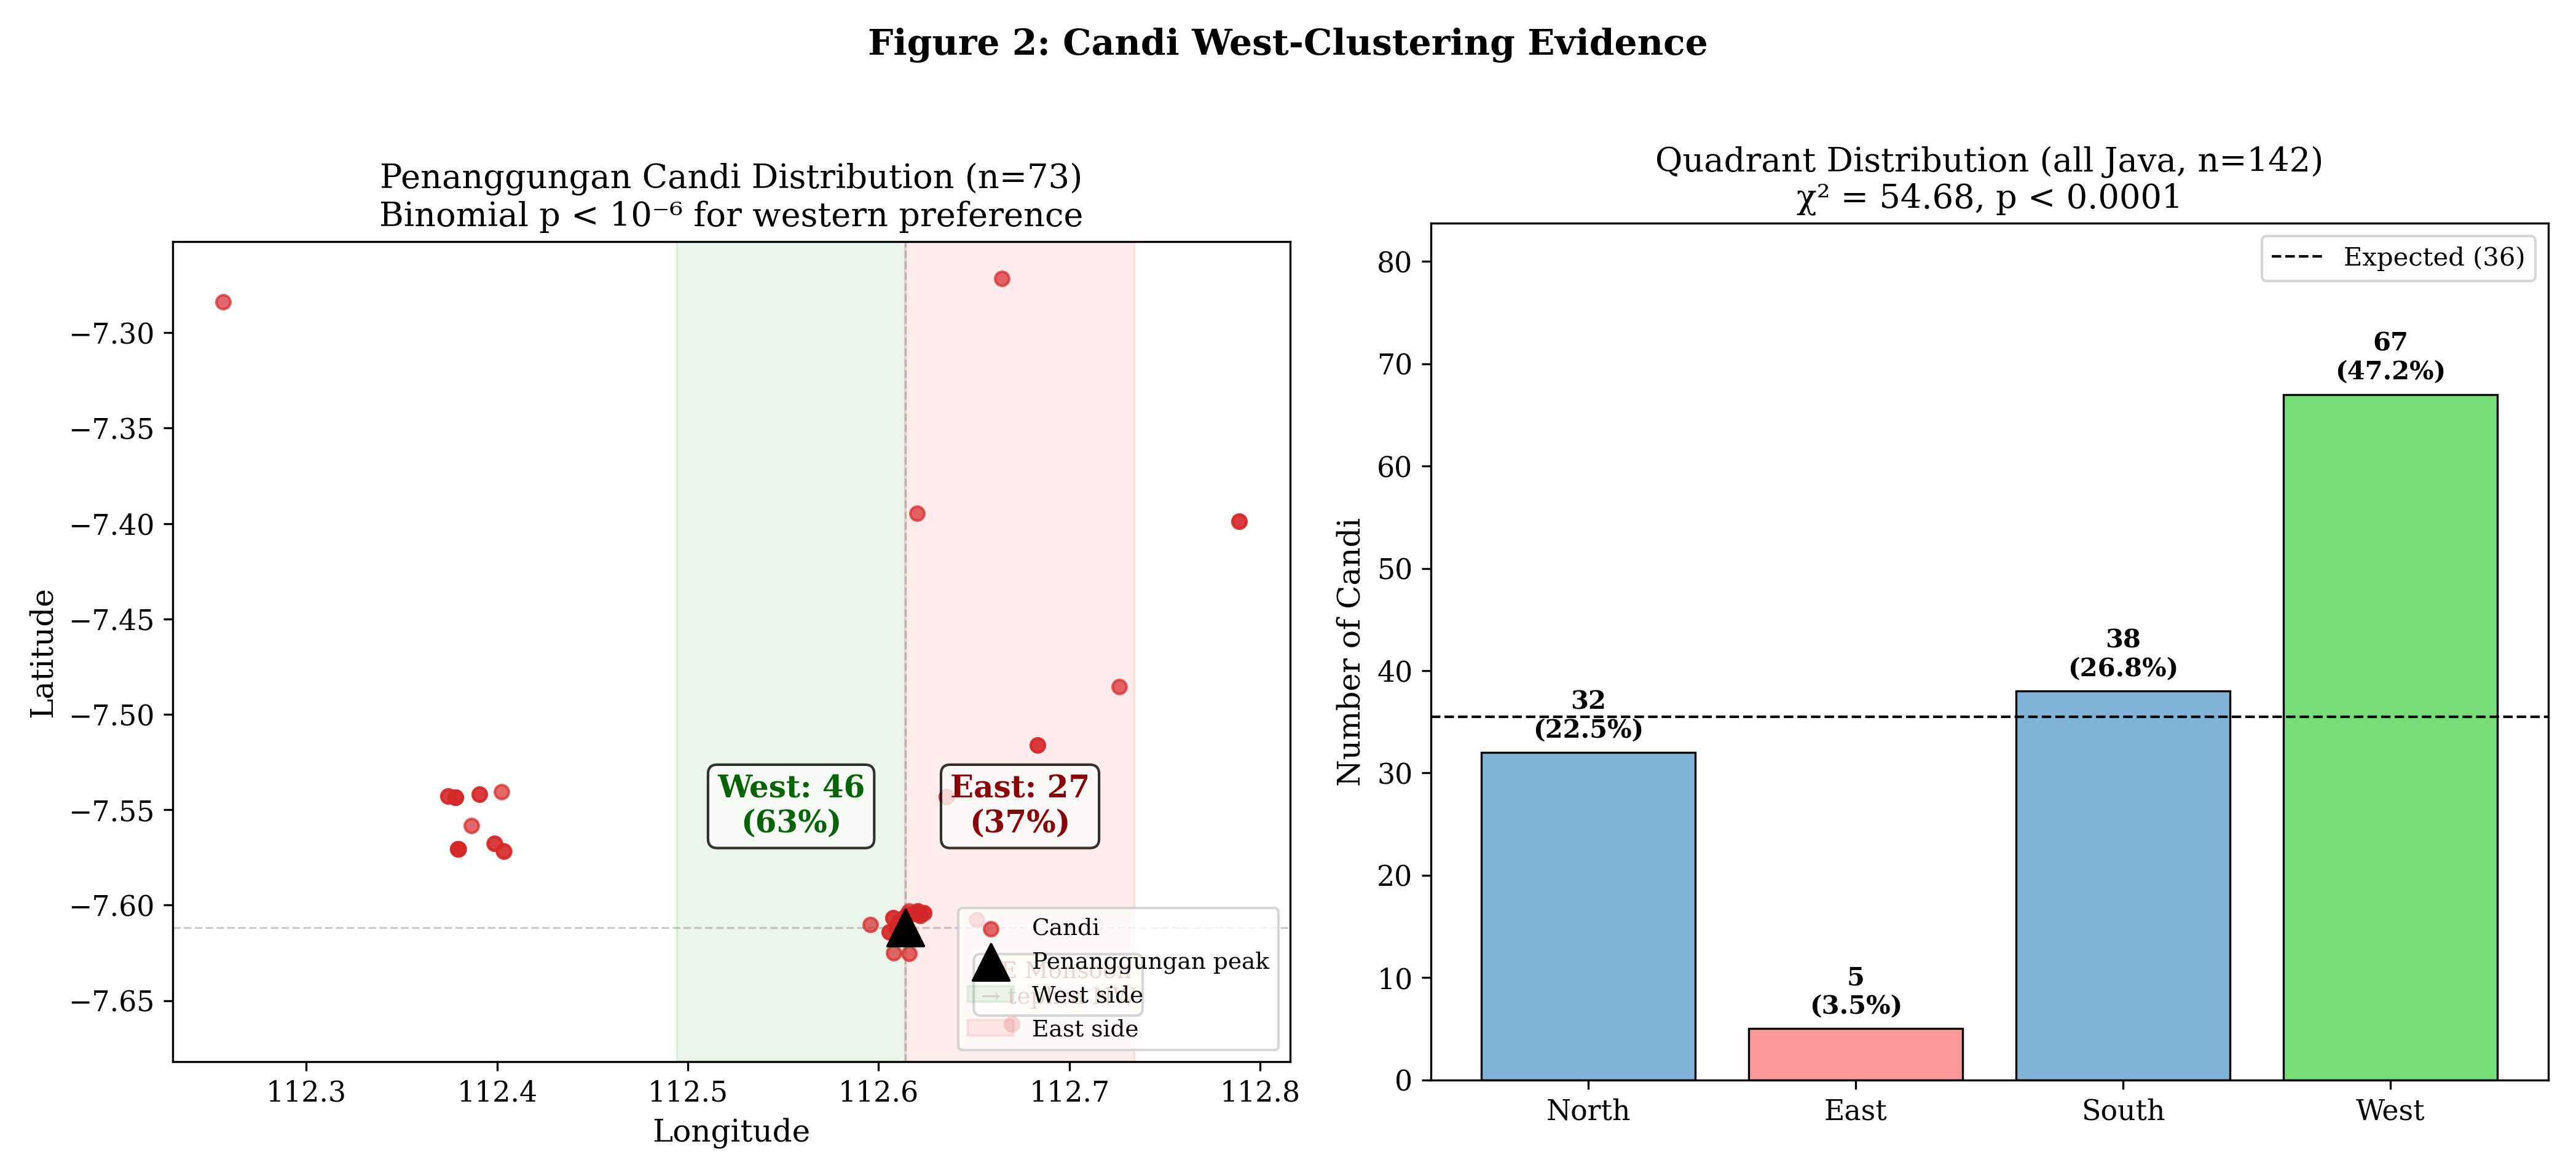
\includegraphics[width=\textwidth]{figures/fig2_penanggungan_westclustering.png}
\caption{Left: Spatial distribution of 73 candi around Penanggungan peak (black triangle). Green shading marks the western side (46 candi, 63\%); red marks the eastern side (27 candi, 37\%). Right: Quadrant distribution for all 142 Java candi. West contains 67 candi (47.2\%), far exceeding the expected 36. East contains only 5 (3.5\%). Dashed line shows expected count under uniform distribution ($\chi^2=54.68$, $p<0.0001$).}
\label{fig:penanggungan}
\end{figure}

\subsubsection{Orientation vs.\ Siting}

Of 20 candi with documented entrance orientation, only 7 (35\%) face toward the nearest volcano---no different from random expectation (binomial $p=0.94$). Entrance orientation follows Hindu canonical prescription (predominantly east-facing), not volcanic direction. This creates a striking contrast: \emph{where} to build is volcanically informed; \emph{how} to orient is religiously determined.

\subsection{Pranata Mangsa Encodes Volcanic Hazard Seasonality}

Eruptions are not uniformly distributed across Pranata Mangsa months (chi-squared $p=0.042$, Rayleigh $p=0.032$). The wet-season month Kapitu (approximately December--January) carries the highest eruption density at 18.14 events per 30-day period, 3.8$\times$ the lowest month Kapat (September; 4.78 per 30-day period).

This monsoon--eruption coupling is physically well-understood: wet-season rainfall infiltrates volcanic edifices, triggering phreatic and phreatomagmatic eruptions. Communities following Pranata Mangsa for agricultural timing---planting decisions, harvest schedules, irrigation management---were thus inadvertently tracking volcanic hazard seasonality. The calendar encodes a dual function: agricultural cycle and volcanic risk indicator.

\begin{figure}[ht]
\centering
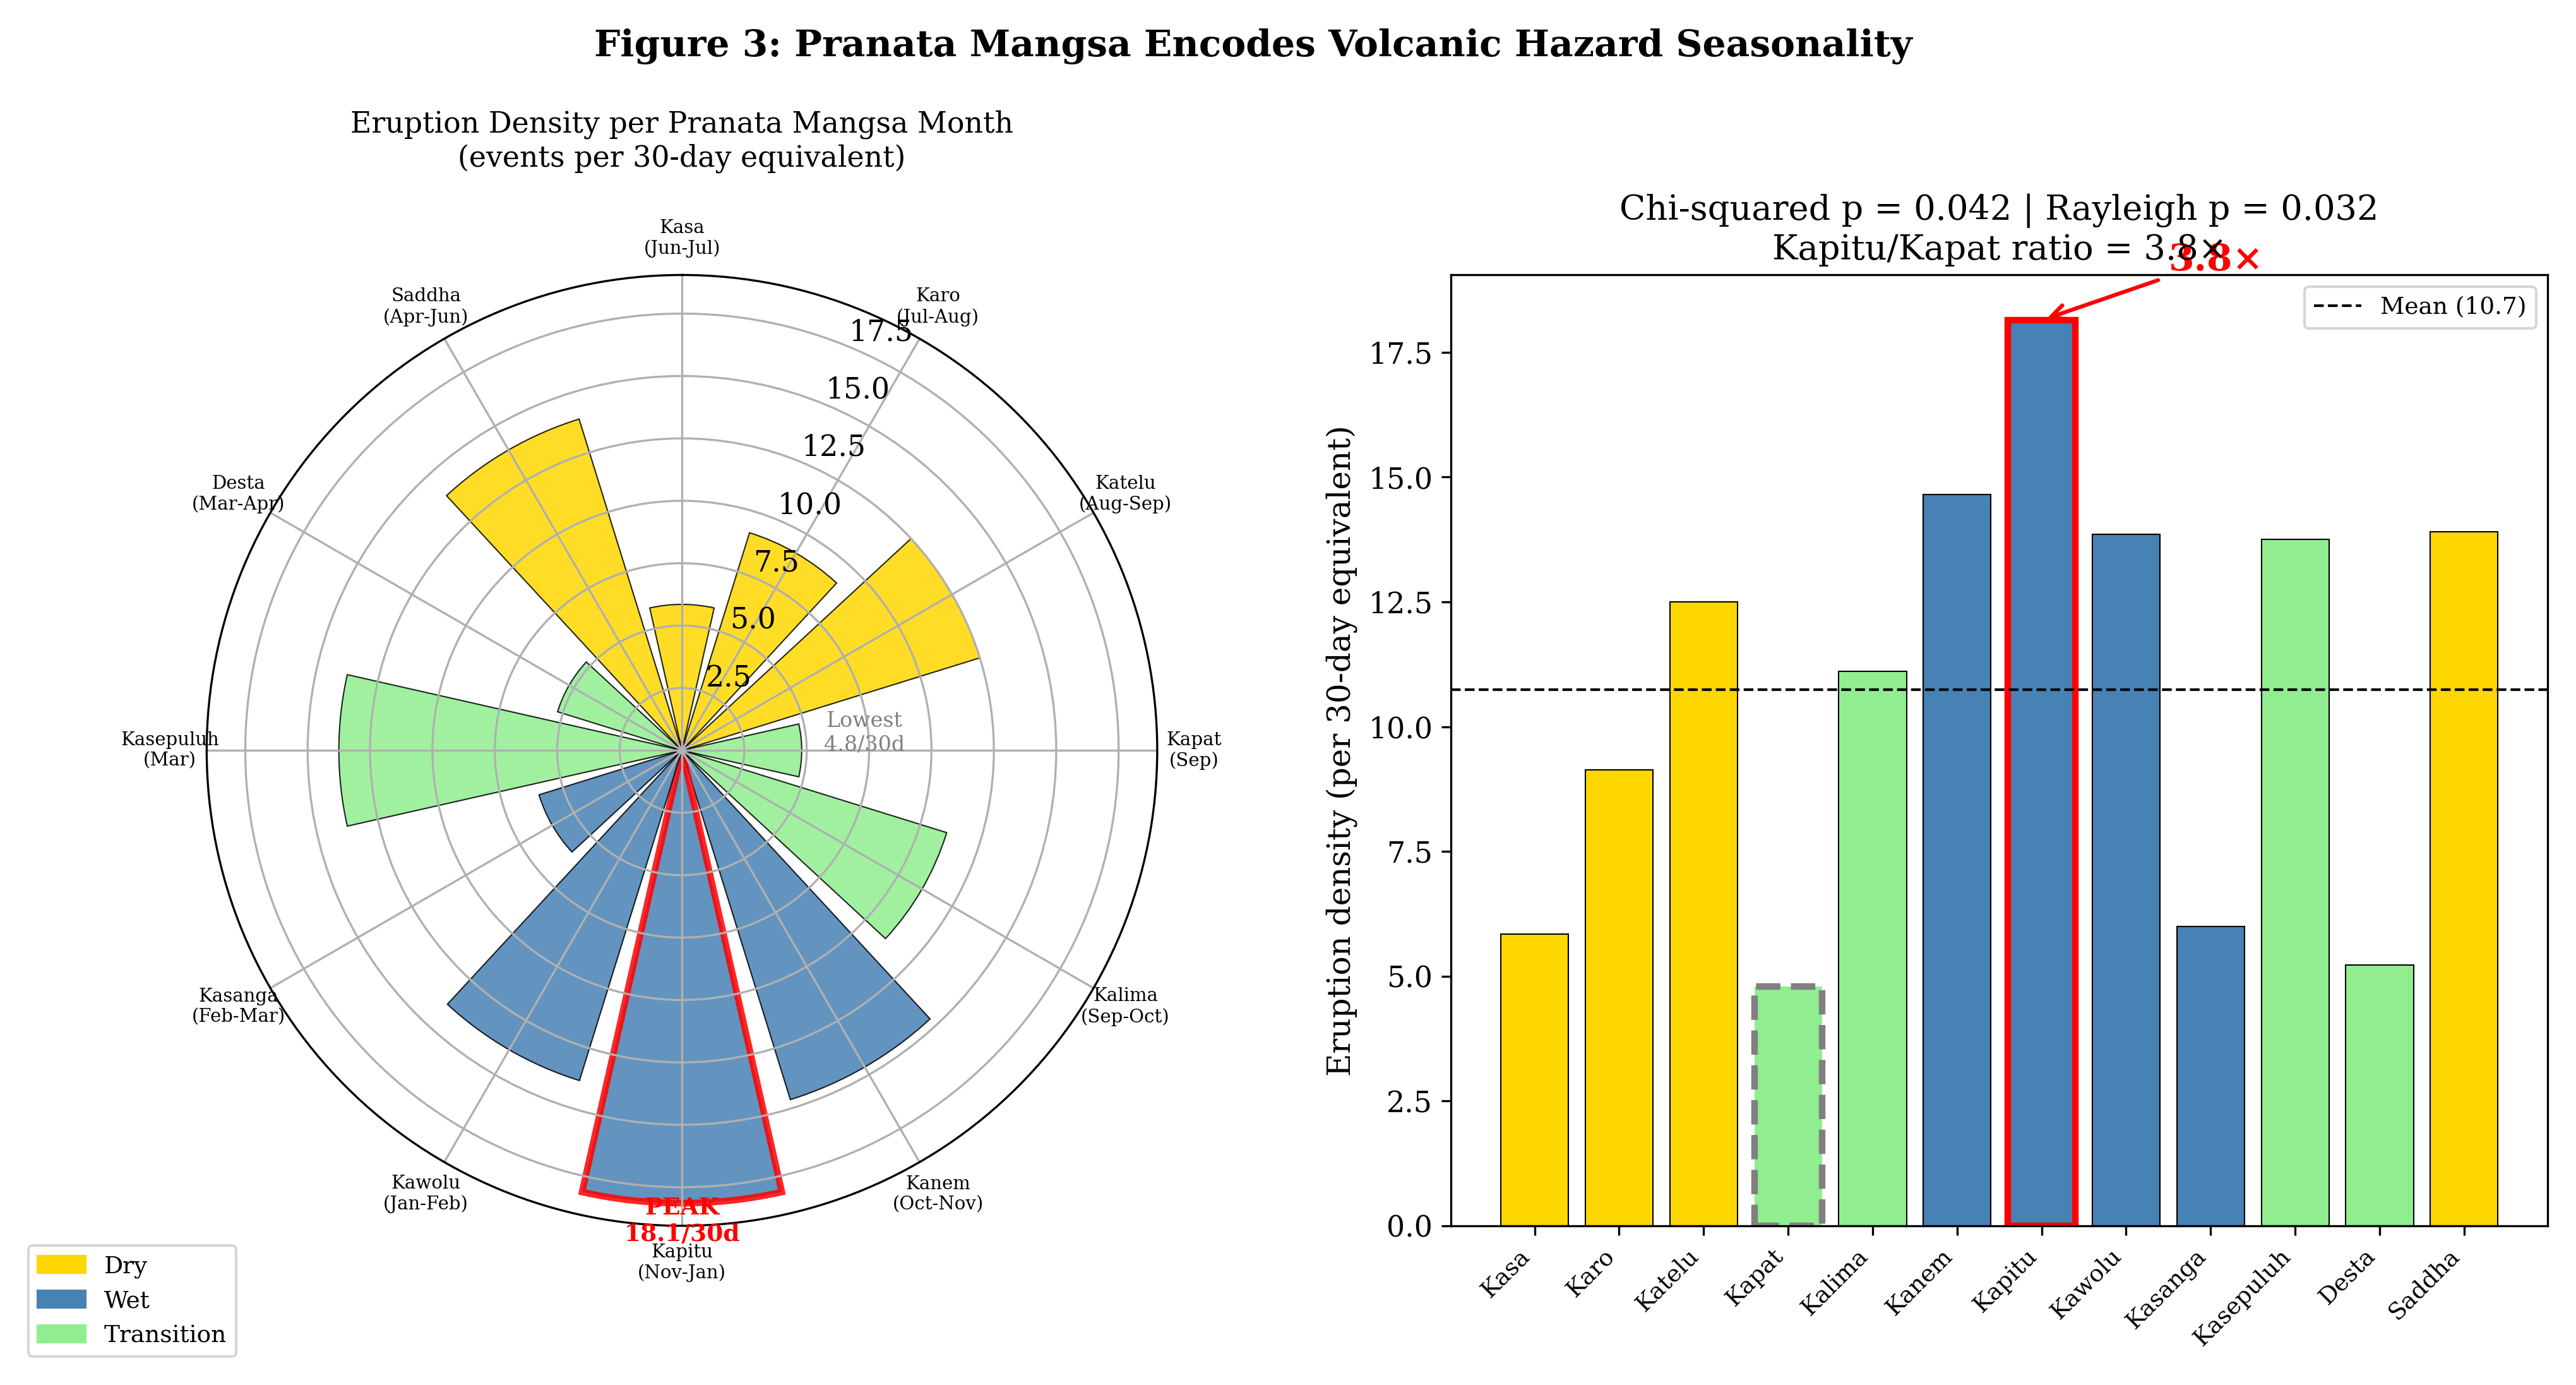
\includegraphics[width=\textwidth]{figures/fig3_eruption_seasonality.png}
\caption{Left: Polar plot of eruption density per Pranata Mangsa month (events per 30-day equivalent). Wet-season months (blue) show highest densities, with Kapitu (Nov--Jan) at 18.1 per 30 days. Dry-season months (yellow) show lowest densities, with Kapat (Sep) at 4.8 per 30 days. Right: Bar chart showing the same data with mean density line. The 3.8$\times$ ratio between Kapitu and Kapat reflects monsoon--eruption coupling (chi-squared $p=0.042$, Rayleigh $p=0.032$).}
\label{fig:seasonality}
\end{figure}

\subsection{Volcanic Informedness Is Local, Not Global}

The three cross-cultural sub-tests consistently reject a global volcanic-cultural correlation:
\begin{itemize}
    \item \textbf{E039a (binary):} No difference between volcanic and non-volcanic islands ($p=0.973$; direction actually \emph{reversed})
    \item \textbf{E039b (continuous):} No correlation between distance to nearest volcano and ritual complexity ($\rho=+0.145$, $p=0.092$; opposite to prediction)
    \item \textbf{E039c (subsistence):} Group hunting ($p=0.002$) and population size ($p=0.010$) do correlate with volcanic proximity, but these reflect volcanic soil fertility and carrying capacity, not cultural selection
\end{itemize}

This constrains the claim: volcanic informedness in Java and Bali is a \emph{local} phenomenon of communities with sustained, proximate volcanic exposure, not a universal consequence of living near volcanoes.

\begin{figure}[ht]
\centering
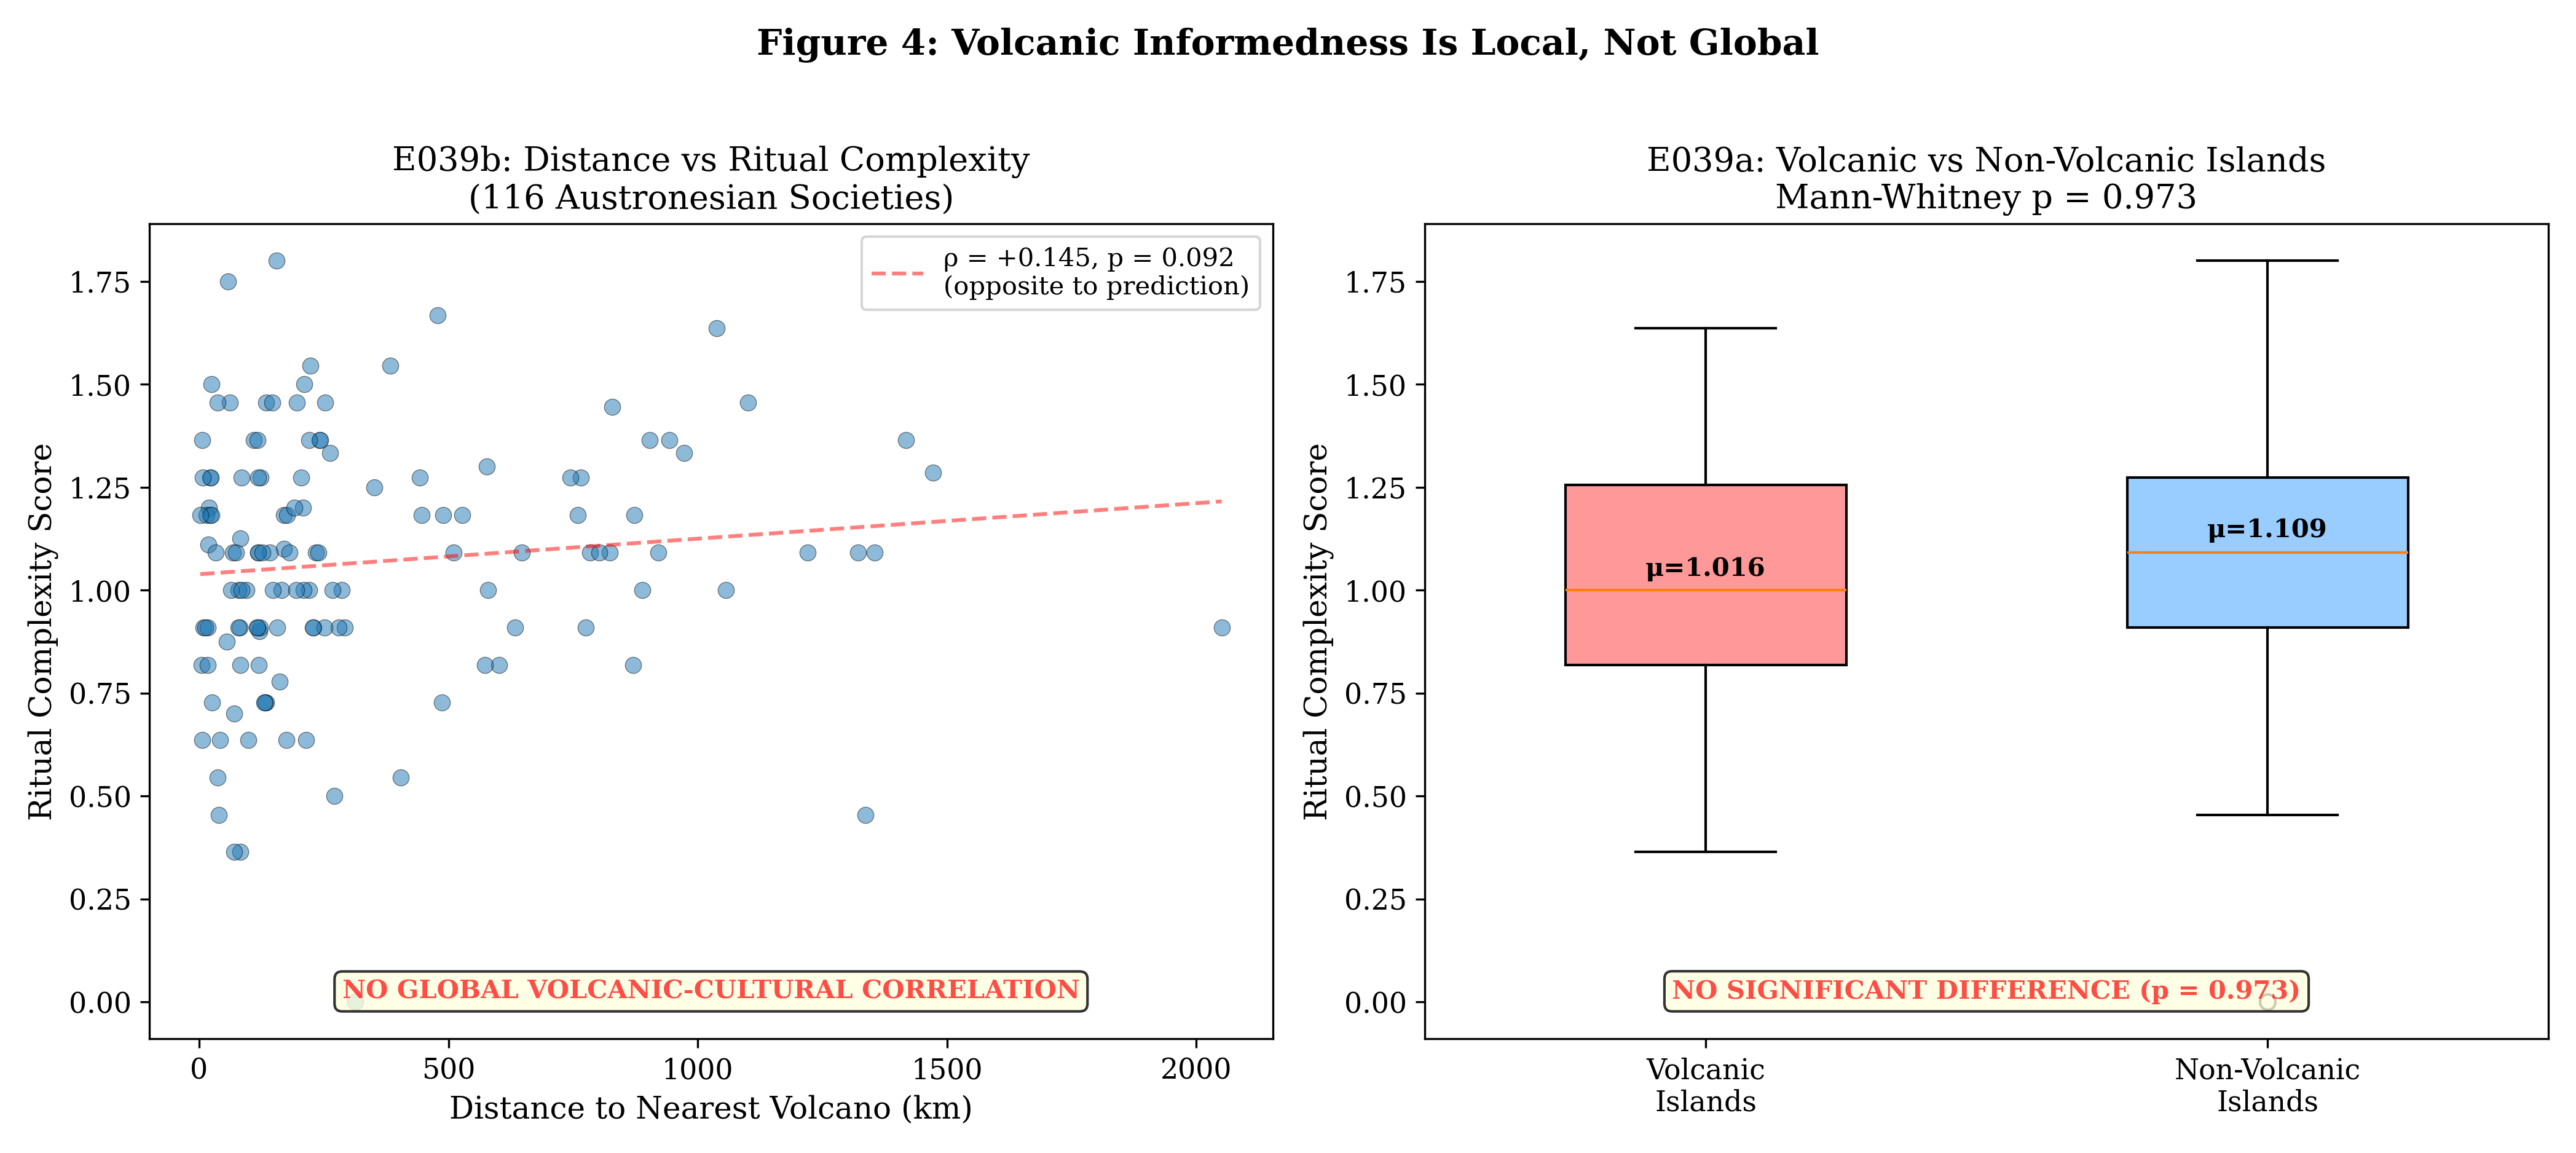
\includegraphics[width=\textwidth]{figures/fig4_crosscultural_falsification.png}
\caption{Cross-cultural falsification of global volcanic-cultural selection. Left: Scatterplot of distance to nearest volcano vs.\ ritual complexity for 116 Austronesian societies. The weak positive correlation ($\rho=+0.145$, $p=0.092$) runs \emph{opposite} to the VCS prediction. Right: Boxplot comparing ritual complexity on volcanic vs.\ non-volcanic islands. No significant difference (Mann-Whitney $p=0.973$). These null results constrain volcanic informedness to a local Java--Bali phenomenon.}
\label{fig:crosscultural}
\end{figure}

\subsection{Toponymic Overwriting: Court-Center, Not Volcanic}

Of 25,244 classified Java village names, 21.7\% were classified as Pre-Hindu, 15.9\% as Sanskrit, 0.3\% as Arabic, 4.9\% as Mixed, and 57.2\% as Unknown. The pre-Hindu ratio varies dramatically by region:

\begin{itemize}
    \item \textbf{Yogyakarta:} 26.2\% pre-Hindu (lowest)---maximum court-center overwriting
    \item \textbf{Madura:} 70--91\% pre-Hindu (highest)---maximum peripheral conservation
    \item \textbf{Overall Java:} 57.7\% pre-Hindu
\end{itemize}

Distance from Yogyakarta (historical court center) significantly predicts pre-Hindu toponymic ratio (Spearman $\rho=0.387$, $p<0.0001$), while distance from nearest volcano does not ($\rho=0.062$, $p=0.511$). Cultural overwriting follows a \emph{court-center} diffusion model, not a volcanic-proximity model.

\subsection{Candi--Toponym Cross-Reference}

\emph{Kabupaten} containing candi have \emph{lower} mean pre-Hindu ratios (0.494) than those without (0.591), a significant difference (Mann-Whitney $U$, $p=0.007$). This indicates that candi cluster in \emph{more} Indianized areas---consistent with both being products of the same Indianization process, but contradicting any hypothesis that volcanic proximity creates a ``preservation zone'' for indigenous toponyms.

% ============================================================
\section{Discussion}
% ============================================================

\subsection{What Volcanic Informedness Is (And Is Not)}

Volcanic informedness, as we have defined and tested it, is:
\begin{itemize}
    \item Practical environmental knowledge encoded in architecture and calendar
    \item Detectable computationally through spatial and temporal distributional analysis
    \item Local to Java and Bali, not pan-Austronesian
\end{itemize}

It is \emph{not}:
\begin{itemize}
    \item Population-level cultural selection (VCS, rejected in Section~4.3)
    \item Deterministic (religious canon overrides volcanic logic for temple orientation)
    \item Unique to Java (analogous patterns may exist in other volcanic cultures, but this was not tested)
\end{itemize}

\subsection{Why Western Siting?}

The western clustering of candi (47.2\%, mean azimuth 279\textdegree) is consistent with two non-exclusive mechanisms:

\begin{enumerate}
    \item \textbf{Tephra sheltering:} The southeast monsoon carries volcanic ash preferentially east and southeast. Western flanks receive less ashfall, making them more suitable for permanent structures.
    \item \textbf{Hydrological advantage:} Orographic rainfall patterns produce more water on western (windward) slopes, supporting denser agricultural populations.
\end{enumerate}

We cannot fully disentangle these mechanisms with the available data. Both predict western clustering, and both represent forms of environmental knowledge. What we can state is that the eastern side of Java's volcanoes---the most exposed to tephra---hosts only 3.5\% of candi, a deficit far exceeding any demographic explanation.

\subsection{Calendar as Environmental Knowledge System}

The Pranata Mangsa calendar is already recognized as a sophisticated Traditional Ecological Knowledge system for agriculture \citep{daldjoeni1984}. Our contribution is demonstrating that this calendar \emph{also} tracks volcanic hazard seasonality, not by design but as a structural consequence of monsoon--eruption coupling.

This finding has implications for disaster risk reduction \citep{lavigne2008}: traditional calendars in volcanic regions may encode hazard information that modern risk assessment systems miss. The 3.8$\times$ eruption density ratio between Kapitu and Kapat represents a significant seasonal concentration that any community following Pranata Mangsa would implicitly ``know''---not as explicit volcanic knowledge, but as heightened awareness of environmental disturbance during specific calendar periods.

\subsection{The VOLCARCH Feedback Loop}

This paper closes a conceptual loop in the VOLCARCH framework:

\begin{enumerate}
    \item Volcanic sedimentation \emph{buries} organic archaeological evidence (Paper 1: sedimentation rates)
    \item This creates a perceived ``blank'' in the pre-Hindu archaeological record (Paper 7: spatial bias)
    \item Scholars fill the blank with external explanations (Indianization, trade contacts)
    \item Endogenous volcanic adaptation is overlooked
    \item The present paper demonstrates that volcanic processes also \emph{shaped} the cultural practices that produced the buried evidence
\end{enumerate}

The feedback is: volcanoes bury the evidence of volcanically-informed cultures, making it appear that these cultures lacked endogenous environmental knowledge. Understanding volcanic informedness is thus essential for correct interpretation of Java's archaeological record.

\begin{figure}[ht]
\centering
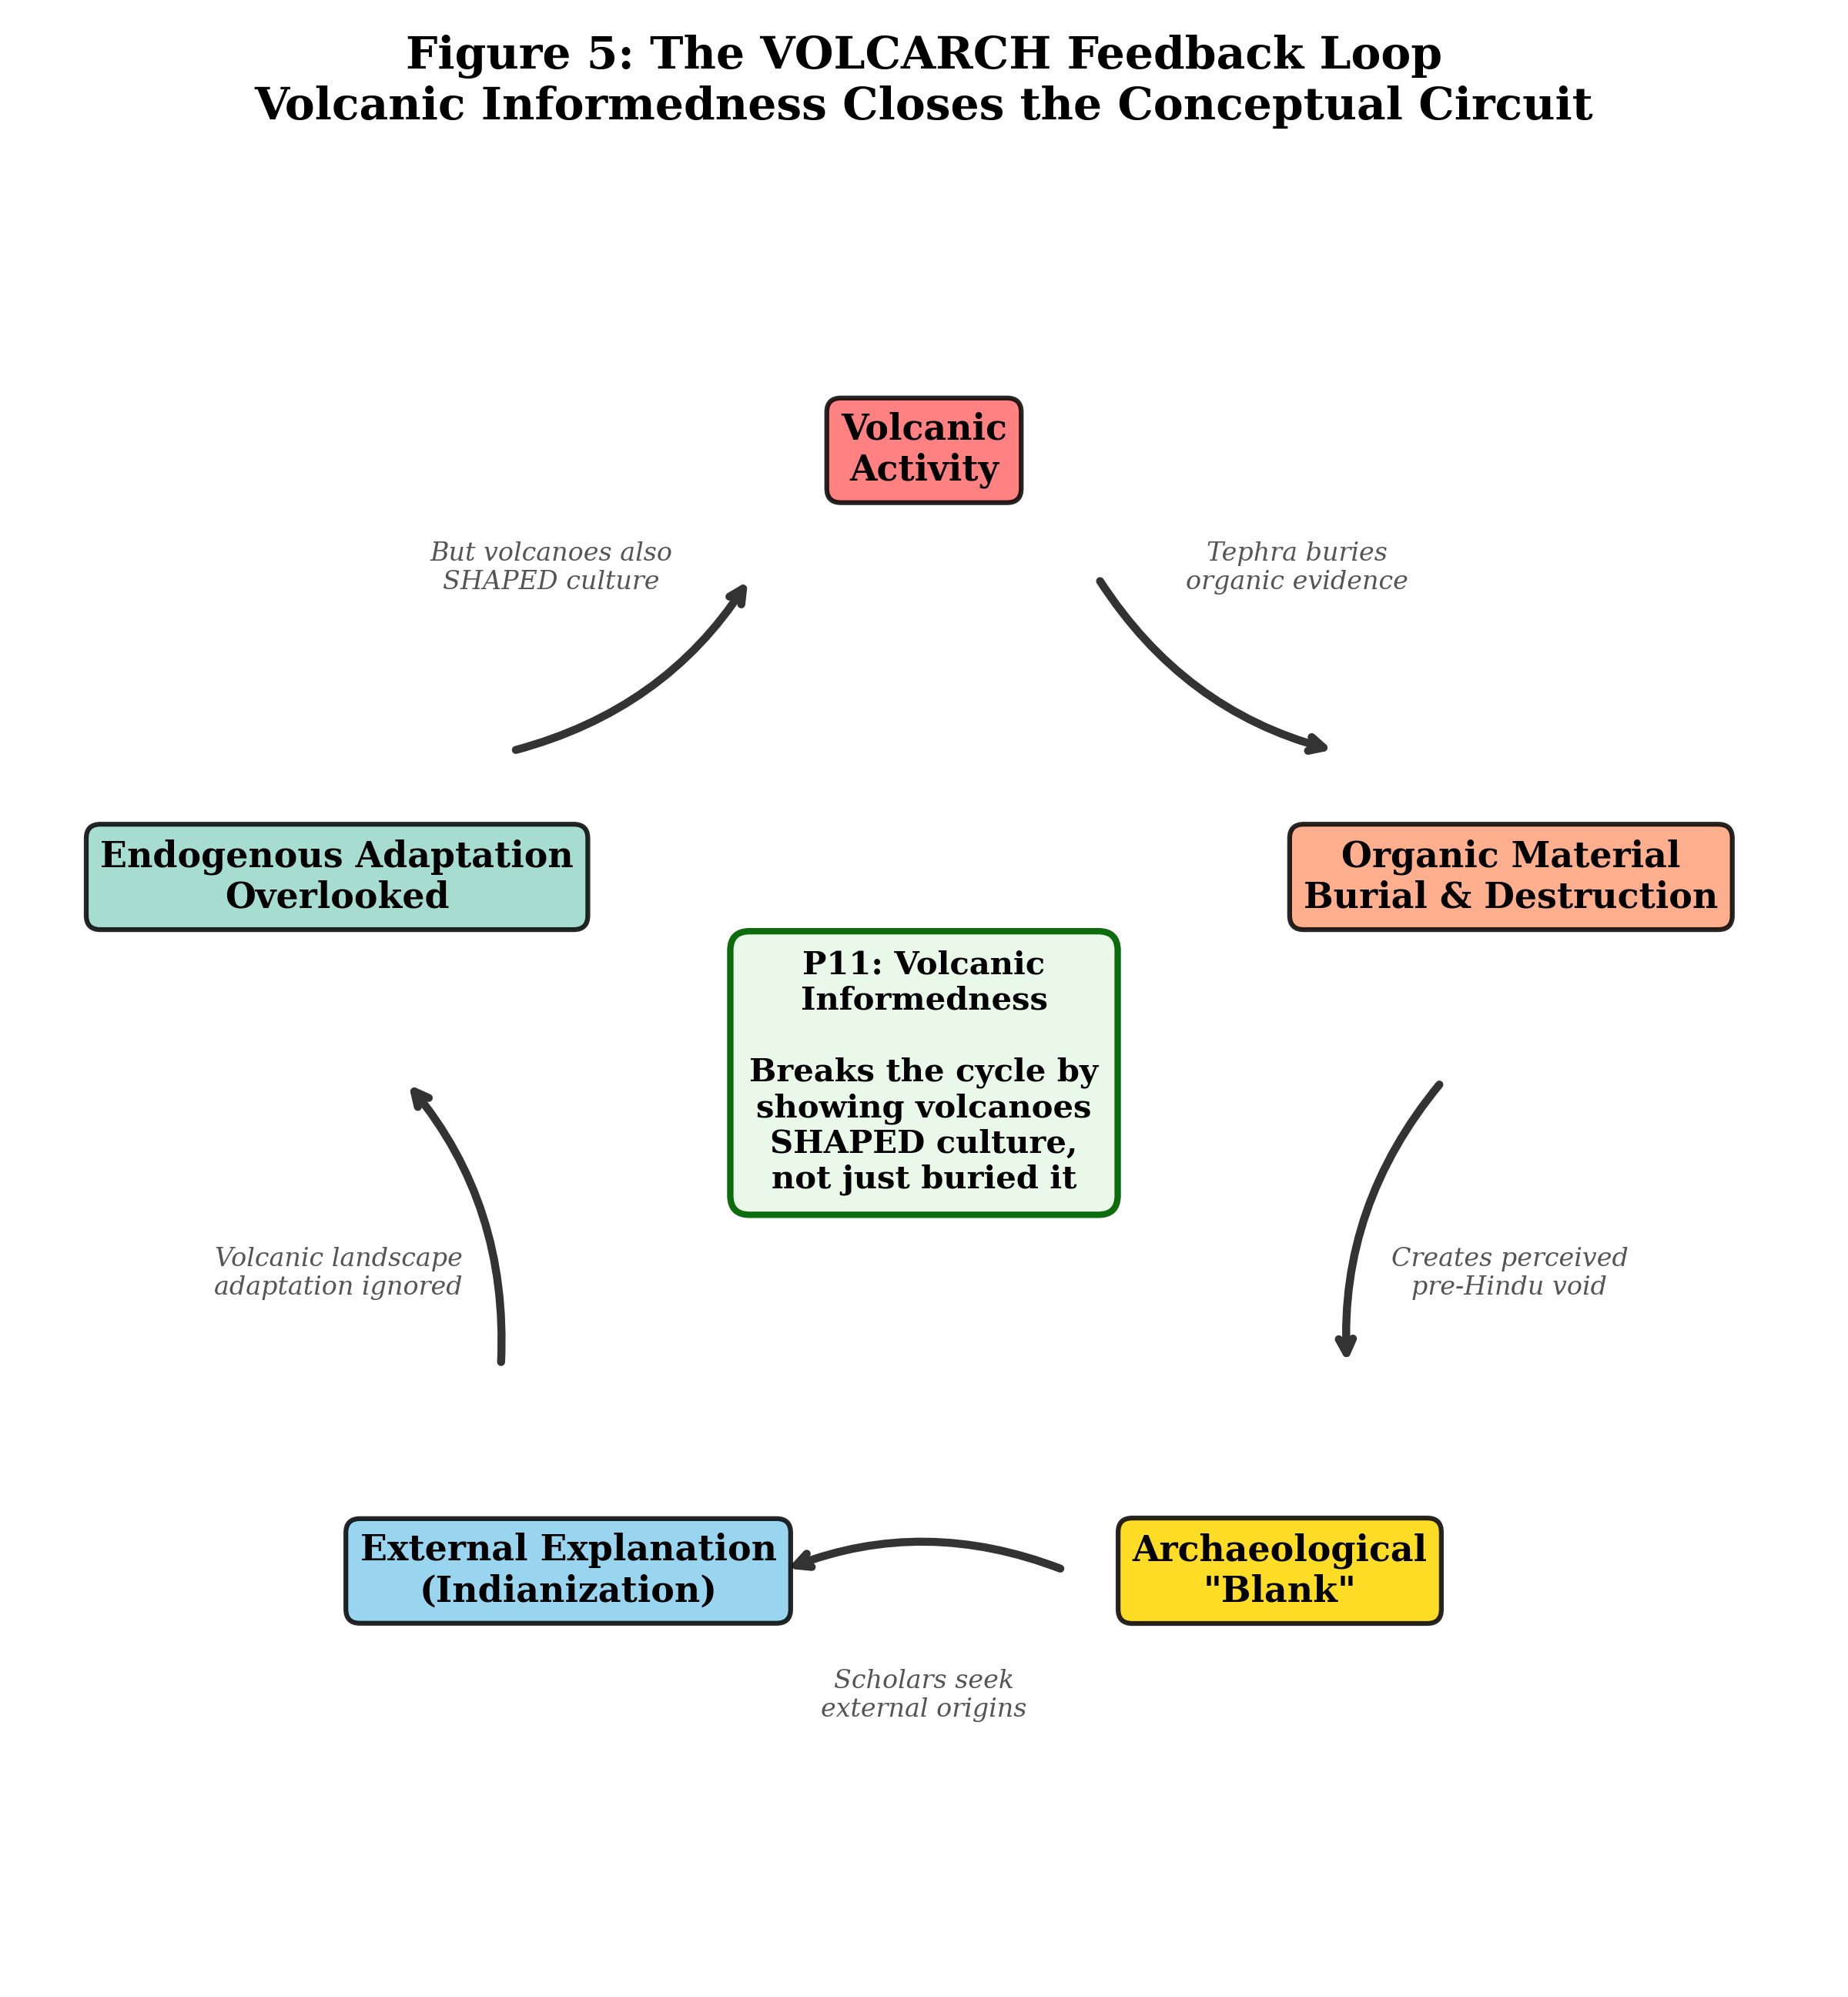
\includegraphics[width=0.75\textwidth]{figures/fig5_feedback_loop.png}
\caption{The VOLCARCH feedback loop. Volcanic activity buries organic evidence (Paper 1), creating a perceived pre-Hindu archaeological blank. Scholars fill this blank with external explanations (Indianization), causing endogenous volcanic landscape adaptation to be overlooked. Paper 11 breaks the cycle by demonstrating that volcanoes also \emph{shaped} the cultural practices that produced the buried evidence.}
\label{fig:feedback}
\end{figure}

\subsection{Limitations}

Several limitations constrain our findings:

\begin{enumerate}
    \item \textbf{Candi sample:} 142 candi, primarily from East Java. Western and Central Java temples (Borobudur, Prambanan) are underrepresented.
    \item \textbf{Eruption data:} Merapi, Java's most active volcano, has potential gaps in the GVP seasonal record.
    \item \textbf{Orientation data:} Only 20 candi have documented entrance directions. A systematic architectural survey would strengthen the siting/orientation distinction.
    \item \textbf{No ethnographic validation:} All evidence is distributional. Interviews with Tengger and Bali Aga communities about volcanic knowledge remain a priority.
    \item \textbf{Population confound:} Western slopes may simply have had more people, independent of volcanic awareness.
    \item \textbf{Toponymic classifier:} 57.2\% of village names classified as ``Unknown'' limits the precision of the toponymic analysis.
\end{enumerate}

% ============================================================
\section{Conclusion}
% ============================================================

Five independent computational tests demonstrate that cultural practices in Java and Bali encode volcanic environmental knowledge:

\begin{enumerate}
    \item Sacred architecture sites preferentially on western (tephra-sheltered) volcanic flanks, with Zone A ($<$10~km) overrepresented by 17.9$\times$
    \item The traditional agricultural calendar inadvertently tracks volcanic hazard seasonality (3.8$\times$ eruption density ratio)
    \item These patterns are local to Java/Bali, not a universal Austronesian trait
    \item Cultural overwriting follows court-center diffusion, not volcanic proximity
    \item Candi and Sanskrit toponyms co-occur, reflecting shared Indianization processes
\end{enumerate}

We term this \emph{volcanic informedness}---the encoding of practical volcanic knowledge in architecture, calendar, and land-use decisions. This local phenomenon of Java and Bali represents a form of Traditional Ecological Knowledge that has been overlooked by archaeological models emphasizing external cultural inputs. Recognizing volcanic informedness is essential both for interpreting the archaeological record and for integrating traditional knowledge into modern volcanic hazard assessment.

% ============================================================
% AI DISCLOSURE
% ============================================================

\subsection*{AI Disclosure}

This research was conducted with the assistance of Claude (Anthropic) for data analysis, statistical testing, and manuscript preparation. All hypotheses, interpretations, and scholarly judgments are those of the human authors. The computational pipeline, including data processing scripts and statistical analyses, is available at the project repository. The use of AI tools enabled a single-researcher operation to function at research-group scale, consistent with emerging norms in computational humanities.

% ============================================================
% REFERENCES (placeholder — will be populated with BibTeX)
% ============================================================

\bibliographystyle{plainnat}
% \bibliography{references}

\begin{thebibliography}{99}

\bibitem[Amien(2026a)]{amien2026p1}
Amien, M. (2026a). Volcanic taphonomic bias in the archaeological record of East Java: A quantitative framework. \emph{Asian Perspectives} (under review).

\bibitem[Amien and Gunawan(2026a)]{amien2026p8}
Amien, M., \& Gunawan, G.F. (2026a). Linguistic fossils: Machine learning detection of pre-Austronesian substrate in western Indonesian languages. \emph{Oceanic Linguistics} (under review).

\bibitem[Amien and Gunawan(2026b)]{amien2026p9}
Amien, M., \& Gunawan, G.F. (2026b). The periphery remembers: Differential conservation of pre-Indic cultural elements in Java, Bali, and Madagascar. \emph{Journal of Southeast Asian Studies} (under review).

\bibitem[Berkes(2018)]{berkes2018}
Berkes, F. (2018). \emph{Sacred Ecology} (4th ed.). Routledge.

\bibitem[Daldjoeni(1984)]{daldjoeni1984}
Daldjoeni, N. (1984). Pranatamangsa, the Javanese agricultural calendar---Its bioclimatological and sociocultural function in developing rural life. \emph{The Environmentalist}, 4(supplement 7), 15--18.

\bibitem[Dumarçay(1993)]{dumarcay1993}
Dumarçay, J. (1993). \emph{The Temples of Java}. Oxford University Press.

\bibitem[GVP(2023)]{gvp2023}
Global Volcanism Program (2023). \emph{Volcanoes of the World}, v. 5.1.1. Smithsonian Institution.

\bibitem[Headley(2004)]{headley2004}
Headley, S.C. (2004). \emph{Durga's Mosque: Cosmology, Conversion, and Community in Central Javanese Islam}. Institute of Southeast Asian Studies.

\bibitem[Lavigne et al.(2008)]{lavigne2008}
Lavigne, F., De Coster, B., Juvin, N., Flohic, F., Gaillard, J.-C., Texier, P., Morin, J., \& Sartohadi, J. (2008). People's behaviour in the face of volcanic hazards: Perspectives from Javanese communities, Indonesia. \emph{Journal of Volcanology and Geothermal Research}, 172(3--4), 273--287.

\bibitem[Marwick(2009)]{marwick2009}
Marwick, B. (2009). Biogeography of Middle Pleistocene hominins in mainland Southeast Asia: A review of current evidence. \emph{Quaternary International}, 202(1--2), 51--58.

\bibitem[Mohr(1938)]{mohr1938}
Mohr, E.C.J. (1938). The relation between soil and population density in the Netherlands East Indies. In \emph{Comptes Rendus du Congr\`{e}s International de G\'{e}ographie}, Amsterdam.

\bibitem[Newhall and Dzurisin(1988)]{newhall1988}
Newhall, C.G., \& Dzurisin, D. (1988). \emph{Historical Unrest at Large Calderas of the World}. U.S. Geological Survey Bulletin 1855.

\bibitem[Riede(2019)]{riede2019}
Riede, F. (2019). \emph{Splendid Isolation: The Eruption of the Laacher See Volcano and Southern Scandinavian Late Glacial Hunter-Gatherers}. Aarhus University Press.

\bibitem[Schlehe(1996)]{schlehe1996}
Schlehe, J. (1996). Reinterpretations of mystical traditions: Explanations of a volcanic eruption in Java. \emph{Anthropos}, 91(4/6), 391--409.

\bibitem[Soekmono(1995)]{soekmono1995}
Soekmono, R. (1995). \emph{The Javanese Candi: Function and Meaning}. Brill.

\bibitem[Stutterheim(1956)]{stutterheim1956}
Stutterheim, W.F. (1956). \emph{Studies in Indonesian Archaeology}. Martinus Nijhoff.

\bibitem[Tanudirjo(1995)]{tanudirjo1995}
Tanudirjo, D.A. (1995). Theoretical trends in Indonesian archaeology. In P. Ucko (Ed.), \emph{Theory in Archaeology: A World Perspective} (pp. 61--75). Routledge.

\bibitem[Thouret(1999)]{thouret1999}
Thouret, J.-C. (1999). Volcanic geomorphology---an overview. \emph{Earth-Science Reviews}, 47(1--2), 95--131.

\bibitem[Watts et al.(2015)]{watts2015}
Watts, J., et al. (2015). Pulotu: Database of Austronesian supernatural beliefs and practices. \emph{PLoS ONE}, 10(9), e0136783.

\bibitem[Whitten et al.(1996)]{whitten1996}
Whitten, T., Soeriaatmadja, R.E., \& Afiff, S.A. (1996). \emph{The Ecology of Java and Bali}. Periplus Editions.

\end{thebibliography}

\end{document}
